\section{Inheritance and Polymorphism}
Vererbung ermöglicht es einer neuen Klasse (Unterklasse oder abgeleiteten Klasse), die Eigenschaften und 
Methoden einer bestehenden Klasse (Oberklasse oder Basisklasse) zu übernehmen.

\begin{minipage}{0.5\columnwidth}
    \begin{itemize}
        \item Code-Wiederverwendung
        \item Modularität
        \item und die Etablierung einer ``is-a''-Beziehung.
    \end{itemize}
\end{minipage}
\begin{minipage}{0.5\columnwidth}
    \begin{center}
        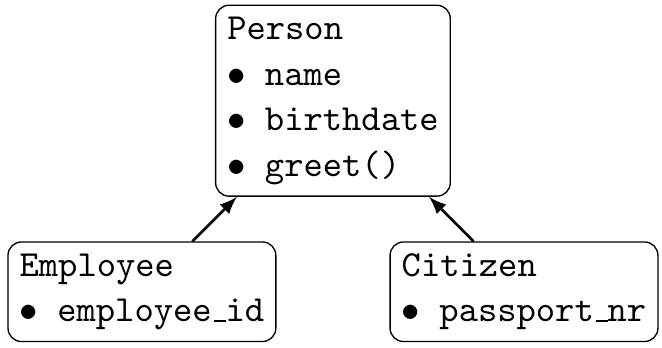
\includegraphics[width=\linewidth]{images/vererbung3.png}
    \end{center}
\end{minipage}\medskip
    
Polymorphie ermöglicht es Unterklassen, Methoden mit demselben Namen wie diejenigen in der Oberklasse zu definieren und sie dadurch effektiv zu überschreiben. Die konkret aufgerufene Methode hängt vom tatsächlichen Objekttyp zur Laufzeit ab und erhöht die Flexibilität der Schnittstelle.

\subsubsection{The \texttt{super()} Function}
Die Funktion \texttt{super()} stellt den Zugriff auf Methoden und Attribute der Oberklasse bereit. Sie wird hauptsächlich innerhalb der Methode \texttt{\_\_init\_\_} der Unterklasse verwendet, um geerbte Attribute zu initialisieren und so sicherzustellen, dass der Basisobjektzustand korrekt eingerichtet wird.

\begin{lstlisting}[language=Python]
class Person:
    def __init__(self, name):
        self.name = name

class Employee(Person):
    def __init__(self, name, employee_id):
        super().__init__(name) # Initialize superclass attributes
        self.employee_id = employee_id
\end{lstlisting}

\subsubsection{Abstract Classes}
Abstrakte Klassen dienen als Vorlagen und können nicht direkt instanziiert werden. Sie definieren abstrakte Methoden, die von abgeleiteten Klassen implementiert werden müssen, wodurch eine konsistente Schnittstelle erzwungen wird. Dafür ist das \texttt{abc}-Modul erforderlich.

\begin{lstlisting}[language=Python]
from abc import ABC, abstractmethod

class Vehicle(ABC):
    @abstractmethod
    def accelerate(self):
        pass

class Car(Vehicle):
    def accelerate(self):
        print('The car accelerates')
\end{lstlisting}

\subsection{Design Principles (SOLID)}
Beim Aufbau von Vererbungshierarchien stellt die Einhaltung von Designprinzipien sicher, dass Flexibilität und Wartbarkeit gewährleistet sind:
\begin{itemize}
    \item \textbf{S}ingle Responsibility: Eine Klasse sollte nur eine Verantwortung haben und für genau eine Sache verantwortlich sein.
    \item \textbf{O}pen-Closed: Klassen sollten für Erweiterungen offen (z. B. über Vererbung) und für Änderungen geschlossen sein.
    \item \textbf{L}iskov Substitution: Objekte einer Oberklasse sollten durch Objekte einer Unterklasse ersetzbar sein, ohne die Korrektheit des Programms zu beeinträchtigen.
    \item \textbf{I}nterface Segregation: Clients sollten nicht dazu gezwungen werden, von nicht verwendeten Methoden abhängig zu sein.
    \item \textbf{D}ependency Inversion: Hochrangige Module sollten nicht von niedrigrangigen Modulen abhängen; beide sollten von Abstraktionen abhängen.
\end{itemize}

\subsection{Aggregation and Composition}
Eine übermäßige Nutzung von Vererbung kann zu dem Problem einer ``class explosion'' führen und erhöht die 
Komplexität erheblich, wenn mehrere Traits oder Optionen kombiniert werden. 

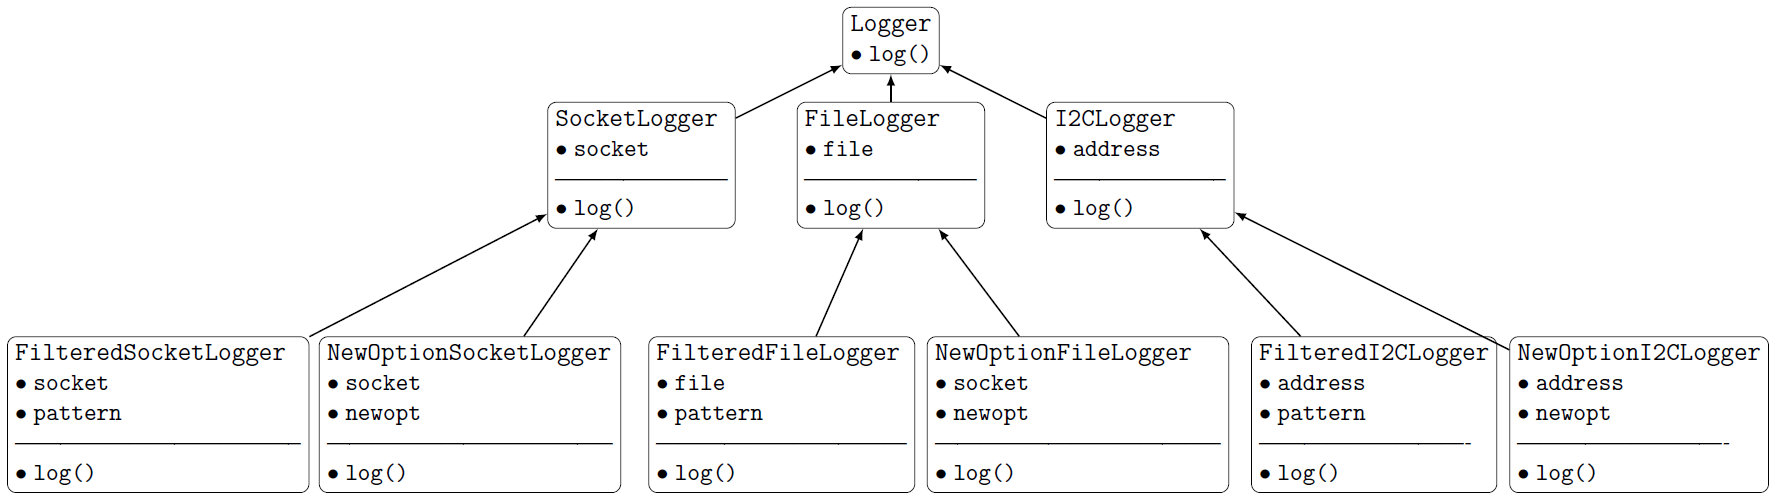
\includegraphics[width=\linewidth]{images/vererbung9.png}

Aggregation und Komposition bieten 
strukturelle Alternativen, indem \textbf{Klassen basierend auf Abhängigkeiten statt auf strikten 
Hierarchien zusammengesetzt werden.}\medskip

\begin{itemize}
    \item \textbf{Komposition (is-a-part-of):} Bedeutet eine starke Lebenszyklus-Abhängigkeit. Das übergeordnete Objekt besitzt und kontrolliert die Lebensdauer der enthaltenen Objekte. Wenn das übergeordnete Objekt zerstört wird, werden auch seine Teile zerstört (z. B. ein Auto und sein Motor).
    \item \textbf{Aggregation (has-a):} Bedeutet eine lose Lebenszyklus-Abhängigkeit. Enthaltene Objekte können unabhängig vom übergeordneten Objekt existieren und können dynamisch hinzugefügt oder entfernt werden (z. B. eine Bibliothek und ihre Bücher).
\end{itemize}

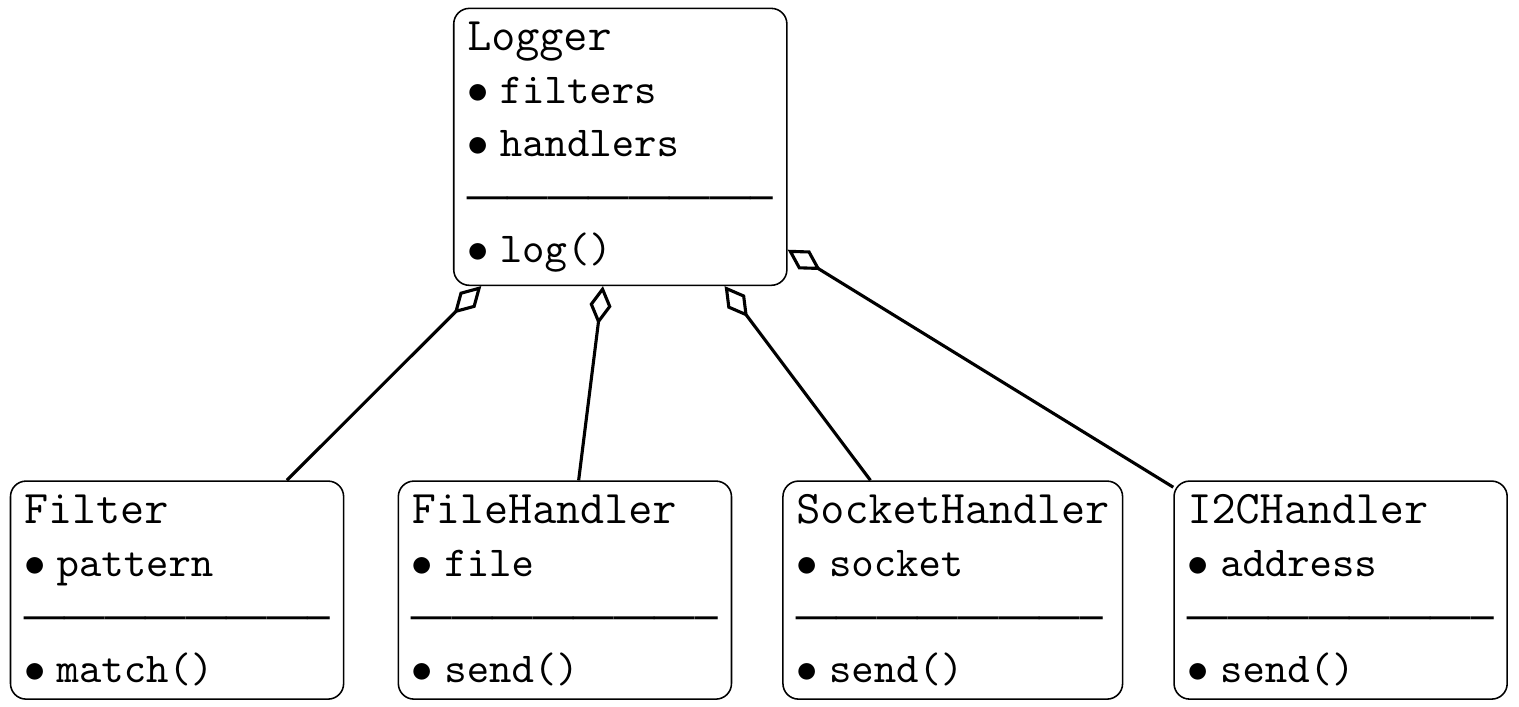
\includegraphics[width=\linewidth]{images/aggregation.png}

\lstinputlisting[language=Python]{code/aggregation.py}